The general equation of second degree is given by
\begin{align}
ax^2+2bxy+cy^2+2dx+2ey+f=0 \label{eq:solutions/41/ex1/gen_quad_eqn}
\end{align}
and can be expressed as
\begin{align}
\vec{x}^T\vec{V}\vec{x}+2\vec{u}^T\vec{x}+f=0 \label{eq:solutions/41/ex1/conic_quad_eqn}
\end{align}
where
\begin{align}
\vec{V} &= \vec{V}^T = \myvec{a & b \\ b & c}
\\
\vec{u}^T &= \myvec{d & e}
\end{align}

Comparing \eqref{eq:solutions/41/ex1/given_curve_eq} with \eqref{eq:solutions/41/ex1/gen_quad_eqn}, we get
\begin{align}
\vec{V} &= \myvec{14  & -2 \\ -2 & 11}
\\
\vec{u}^T &= \myvec{-22 & -29}
\end{align}
If $\abs{\vec{V}} > 0$, then \eqref{eq:solutions/41/ex1/conic_quad_eqn} is an ellipse. 
\begin{align}
\abs{V} = \mydet{14 & -2 \\ -2 & 11} = 150 > 0 \label{eq:solutions/41/ex1/ellipse_proved_eq}
\end{align}
\eqref{eq:solutions/41/ex1/conic_quad_eqn} can be expressed as
\begin{align}
\label{eq:solutions/41/ex1/conic_simp_temp_nonparab_eq}
\vec{y}^T\vec{D}\vec{y} &=  \vec{u}^T\vec{V}^{-1}\vec{u} -f  &  \abs{V} &\ne 0
\\
\vec{y}^T\vec{D}\vec{y} &=  -\eta\myvec{1 & 0}\vec{y}   & \abs{V} &= 0
\label{eq:solutions/41/ex1/conic_simp_temp_parab_eq}
\end{align}
with center as 
\begin{align}
    \vec{c} &= - \vec{V}^{-1}\vec{u} & \abs{V} &\ne 0
\end{align}
Calculating the center for given curve we get,
\begin{align}
    \vec{c} &= - \frac{1}{\abs{14\times11 - \brak{-2\times-2}}}\myvec{11  & 2 \\ 2 & 14}\myvec{-22 \\ -29} \\
    &= \frac{1}{150}\myvec{300 \\ 450} \\
    &= \myvec{2 \\ 3}
\end{align}
For 
\begin{align} 
\abs{\vec{V}} > 0, \quad \text{or, } \lambda_1 > 0, \lambda_2 > 0 
\end{align} 
\eqref{eq:solutions/41/ex1/conic_simp_temp_nonparab_eq} becomes 
\begin{align} \lambda_1y_1^2 +\lambda_2y_1^2 = 
\vec{u}^T\vec{V}^{-1}\vec{u} -f 
\end{align} 
which is the equation of an ellipse with major and minor axes 
parameters
\begin{align} 
\sqrt{\frac{\lambda_1}{\vec{u}^T\vec{V}^{-1}\vec{u} -f}}, 
\sqrt{\frac{\lambda_2}{\vec{u}^T\vec{V}^{-1}\vec{u} -f}} \label{eq:solutions/41/ex1/axes_eq}
\end{align}
The characteristic equation of $\vec{V}$ is obtained by evaluating the determinant
\begin{align}
\mydet{\lambda \vec{I}-\vec{V}} = \mydet{\lambda -14 & 2 \\ 2 & \lambda -11} &= 0
\\
\implies \lambda^2 - 25\lambda + 150 &= 0
\label{eq:solutions/41/ex1/ellipse_char_eq}
\end{align}
The eigenvalues are the roots of \eqref{eq:solutions/41/ex1/ellipse_char_eq} given by
\begin{align}
\lambda_1 = 15, \lambda_2 = 10
\label{eq:solutions/41/ex1/ellipse_eval_eq}
\end{align}
The eigenvector $\vec{p}$ is defined as
\begin{align}
\vec{V} \vec{p}&= \lambda \vec{p}
\\
\implies \brak{\lambda\vec{I}-\vec{V}}\vec{p} &=0
\end{align}
where $\lambda$ is the eigenvalue.  For $\lambda_1 = 15$,
\begin{align}
\brak{\lambda_1\vec{I}-\vec{V}}
= \myvec{1 & 2 \\ 2 & 4} 
\xleftrightarrow{R_2\leftarrow R_2-2R_1}\myvec{1 & 2 \\0 & 0 }  
\\
\implies \vec{p}_1 = \frac{1}{\sqrt{5}}\myvec{2 \\ -1}
\end{align}
such that $\norm{\vec{p}_1} = 1$.  Similarly, the eigenvector corresponding to $\lambda_2$ can be obtained as
\begin{align}
 \vec{p}_2 = \frac{1}{\sqrt{5}}\myvec{1 \\ 2}
\end{align}
It is easy to verify that 
\begin{align}
\vec{V} &= \vec{P}\vec{D}\vec{P}^{-1}=\vec{P}\vec{D}\vec{P}^T \quad \because \vec{P}^{-1} = \vec{P}^{T} \label{eq:solutions/41/ex1/ellipse_spectrum_eq}
\\
\text{or, } \vec{D} &= \vec{P}^T\vec{V}\vec{P}
\end{align}
where 
\begin{align}
\vec{P} & =\myvec{\vec{p}_1 & \vec{p}_2} = \frac{1}{\sqrt{5}}\myvec{2 & 1\\ -1 & 2} \label{eq:solutions/41/ex1/ellipse_spectrum_P_eq}
\\
 \vec{D} &= \myvec{\lambda_1 & 0 \\ 0 & \lambda_2} =\myvec{15 & 0\\ 0 & 10}
\label{eq:solutions/41/ex1/eq:ellipse_spectrum_D}
\end{align}
Calculating the ellipse parameters using \eqref{eq:solutions/41/ex1/axes_eq}, we get
\begin{align}
\vec{u}^T\vec{V}^{-1}\vec{u} &= \nonumber \\
&= \myvec{-22 -29}\frac{1}{150}\myvec{11 & 2 \\ 2 &1 4 }\myvec{-22 \\ -29} \nonumber \\
&= \frac{1}{150}\myvec{300 & 450}\myvec{22 \\ 29} \nonumber \\
&= 131 \nonumber \\
\vec{u}^T\vec{V}^{-1}\vec{u} -f &= 131 - 71 = 60 \\
\sqrt{\frac{\vec{u}^T\vec{V}^{-1}\vec{u} -f}{\lambda_1}} &= \sqrt{\frac{60}{15}} = 2 \\
\sqrt{\frac{\vec{u}^T\vec{V}^{-1}\vec{u} -f}{\lambda_2}} &= \sqrt{\frac{60}{10}} = \sqrt{6}
\end{align}

Thus, the given curve is found to be an ellipse from \eqref{eq:solutions/41/ex1/ellipse_proved_eq} with center at $\myvec{2 & 3}$ and the major and minor axes lengths are calculated as $\sqrt{6}$, $2$. An ellipse with these parameters along with one having center as origin are plotted as shown.

\begin{figure}[!ht]
\centering
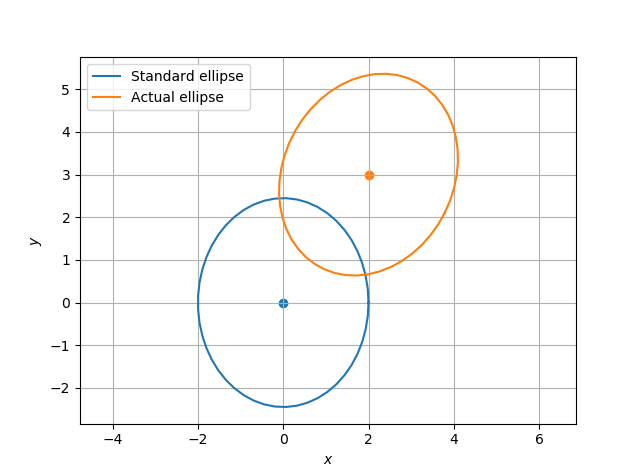
\includegraphics[width=\columnwidth]{./solutions/41/ex1/assignment_6_figure.png}
\caption{Ellipse with center (2 3) and having the axes lengths as $\sqrt{6}$ and 2 along with an ellipse with center as origin}
\label{eq:solutions/41/ex1/Fig:Ellipse}
\end{figure}
